\documentclass[
a4paper,
oneside,
10pt,
fleqn,
headsepline,
toc=listofnumbered, 
bibliography=totocnumbered]{scrartcl}

% deutsche Trennmuster etc.
\usepackage[T1]{fontenc}
\usepackage[utf8]{inputenc}
\usepackage[english, ngerman]{babel} % \selectlanguage{english} if  needed
\usepackage{lmodern} % use modern latin fonts

% Custom commands
\newcommand{\AUTHOR}{Michael Wieland}
\newcommand{\SECONDAUTHOR}{Fabian Hauser}
\newcommand{\INSTITUTE}{Hochschule für Technik Rapperswil}

% Jede Überschrift 1 auf neuer Seite
\let\stdsection\section
\renewcommand\section{\clearpage\stdsection}

% Multiple Authors
\usepackage{authblk}

% Include external pdf
\usepackage{pdfpages}

% Layout / Seitenränder
\usepackage{geometry}

% Inhaltsverzeichnis
\usepackage{makeidx} 
\makeindex

\usepackage{url}
\usepackage[pdfborder={0 0 0}]{hyperref}
\usepackage[all]{hypcap}
\usepackage{hyperxmp} % for license metadata

% Mathematik
\usepackage{amsmath}
\usepackage{amssymb}
\usepackage{amsfonts}
\usepackage{enumitem}

% Images
\usepackage{graphicx}
\graphicspath{{images/}} % default paths

% Boxes
\usepackage{fancybox}

%Tables
\usepackage{tabu}
\usepackage{booktabs} % toprule, midrule, bottomrule
\usepackage{array} % for matrix tables

% Multi Columns
\usepackage{multicol}

% Header and footer
\usepackage{scrlayer-scrpage}
\setkomafont{pagehead}{\normalfont}
\setkomafont{pagefoot}{\normalfont}
\automark*{section}
\clearpairofpagestyles
\ihead{\headmark}
\ohead{\TITLE}
\cfoot{\pagemark}

% Pseudocode
\usepackage{algorithm}
\usepackage{algorithmic}

% Code Listings
\usepackage{listings}
\usepackage{color}
\usepackage{beramono}

\definecolor{DarkPurple}{rgb}{0.4, 0.1, 0.4}
\definecolor{DarkCyan}{rgb}{0.0, 0.5, 0.4}
\definecolor{LightLime}{rgb}{0.3, 0.5, 0.4}
\definecolor{Blue}{rgb}{0.0, 0.0, 1.0}

\lstdefinestyle{eclipse-style}{
	language=Java,  
	columns=flexible,
	showstringspaces=false,     
	basicstyle=\footnotesize\ttfamily, 
	keywordstyle=\bfseries\color{DarkPurple},
	commentstyle=\color{LightLime},
	stringstyle=\color{Blue}, 
	escapeinside={£}{£}, % latex scope within code      
	morekeywords={length},
	numbers=left,
	numberstyle=\tiny\color{black},
	frame=single,
}
\lstset{style=eclipse-style}


% Theorems \begin{mytheo}{title}{label}
\usepackage{tcolorbox}
\tcbuselibrary{theorems}
\newtcbtheorem[number within=section]{definiton}{Definition}%
{fonttitle=\bfseries}{def}
\newtcbtheorem[number within=section]{remember}{Merke}%
{fonttitle=\bfseries}{rem}
\newtcbtheorem[number within=section]{hint}{Hinweis}%
{fonttitle=\bfseries}{hnt}

% Dokumentinformationen
\newcommand{\SUBJECT}{Report}
\newcommand{\TITLE}{Cloud Infrastructre Lab 3}

\begin{document}
	
% Front page
\title{\TITLE}
\subject{\SUBJECT}
\author{\SECONDAUTHOR}
\author{\AUTHOR}
\affil{\INSTITUTE}
\date{\today}
\maketitle

% Table of contents
\tableofcontents


% 14.10.2016, 23:55, as PDF to beat.stettler@ins.hsr.ch

\section{Datacenter Design}

\subsection{Grundlegendes}
Wie auch im Campus Network wird auch das Datacenter in drei Layer unterteilt. 
\begin{description}
	\item[Access Layer] \hfill \\
	Verbindet die Endgeräte mit dem weiteren Netzwerk. Regelt Port Security, VLAN's und PoE.
	\item[Aggregation Layer] \hfill \\
	Switches fassen Datenströme aus dem Access Layer zusammen. Regelt das Routing zwischen den VLANs und QoS.
	\item[Core Layer] \hfill \\
	Regelt den Verkehr im Backbone
\end{description}

\subsection{Anforderungen}
Für die Firma BetaHouse Inc. muss ein hochverfügbares, skalierbares und redundantes Datacenter designed werden, welches Platz für folgende Geräte bietet.
\begin{table}[h]
	\centering
	\begin{tabu}{l l l}
		\toprule
		Anzahl & Typ & Bereich \\
		\midrule
		30 & Server & IT \\
		30 & Server & HR \\
		30 & Server & Trading \\
		2  & Core Switch & Core Tier \\
		3  & Aggregation Switch & Aggregation Tier \\
		6  & Access Switch & Access Tier \\
		\bottomrule
	\end{tabu}
	\caption{Server und Switches}
\end{table}

\subsubsection{Sicherheit}
Die einzelnen Netze der Abteilungen müssen strikt getrennt werden. Es darf keine Konnektivität zwischen den Abteilungen ohne explizite Ausnahme stattfinden.

\subsubsection{Verfügbarkeit und Redundanz}
In Punkto Ausfallsicherheit wird ein Tier-3 Datacenter angestrebt, was eine Verfügbarkeit von 99.982\% verspricht. Das Datencenter muss rund um die Uhr betriebsbereit zur Verfügung stehen und Wartungen müssen unbemerkt bleiben. Das Netzwerk besteht aus mehreren Pfaden, wobei durch STP immer nur ein Pfad aktiv verwendet wird.  
\begin{table}[h]
	\centering
	\begin{tabu}{l l}
		\toprule
		Beschreibung & Anforderung \\
		\midrule
		Versorgungswege Elektro/Kühlung & 1 aktiv, 1 passiv \\
		Redundanz Aktivkomponenten & N + 1 \\
		Backbone Redundanz & ja\\
		Redundanz Horizontaltverkabelung & nein\\
		USV und Generator & ja\\
		Unterbruchsfreie Wartung & ja\\
		Verfügbarkeit & 99.982\% \\
		\bottomrule
	\end{tabu}
	\caption{Tier 3 Infrastruktur}
\end{table}

\paragraph{Geo Redundanz}
Bei Datacenter von diesem Umfang, sollte eine geografische Redundanz in Betracht gezogen werden. Dabei wird ein zweites Datacenter an einem anderen Standort aufgebaut. Im Fehlerfall kann auf dieses umgeschalten werden. 

\subsection{Skalierbarkeit}
Das Datacenter sollte so skalierbar sein, dass es dem Wachstum einer Firma nachkommen kann. Dies bedingt den Einsatz eines Core Layers, damit der Aggregation Layer ohne weiteres ausgebaut werden kann.

\subsubsection{Infrastruktur}
Ein Datacenter stellt naturgemäss folgende Anforderungen an die Gebäudeinfrastruktur.
\begin{itemize}
	\item Geeignetes Kühlungssystem
	\item Schutz gegen Stromausfälle mittels USV und Dieselgeneratoren
	\item Erdung und Schutz gegen Spannungsschwankungen
	\item Zugangsschutz gegen unerlaubten Zutritt
	\item Schutz gegen externe Gefahrenfaktoren wie Naturkatastrophen, Luftverkehr und andere Gefahren die von der Umgebung ausgehen können.
\end{itemize}

\subsubsection{Core Layer}
Im Core Layer geht es im speziellen um die Geschwindigkeit sowie Hochverfügbarkeit und Redundanz. Da im Core die Daten des Aggregation Layer zusammengefasst werden, müssen grosse Datenmengen performant verarbeitet werden können. Dadurch entstehen hohe Betriebstemperaturen, weshalb die Geräte im Core permanent herunter gekühlt werden müssen.

\subsubsection{Verkabelung}
Bei der Verkabelung wird bis zu den Access Switches Glasfasern eingesetzt. Um Kosten zu sparen werden die Server aber mit Kupferkabel angeschlossen.

\subsubsection{Server}
Auch bei den Server ist Redundanz gefordert, weshalb alle Server über 5 Anschlüsse verfügen müssen. 
\begin{itemize}
	\item 2 für das LAN 
	\item 2 für das SAN (Fibre Channel übers Glas oder FCoE)
	\item 1 für KVM (Keyboard/Video/Mouse)
\end{itemize}

\subsection{Physisches Design}
Die Netzwerkgeräte werden gemäss der Top of Rack (ToR) Architektur organisiert. Diese eignet sich insbesondere für Hochgeschwindigkeitsverbindungen, welche im Highfrequency Trading gefordert sind. Mit der gewählten Architektur können 10Gib-Ethernet Anforderungen leicht bewältigt werden. Im oberen Bereich eines jeden Racks wird ein Access Switch positioniert. Die Architektur bietet klare Vorteile:
\begin{itemize}
	\item kleineres Kabelvolumen, was das System wartbarer macht. Zusätzlich sind die Installationskosten geringer
	\item geeignet für hohe Serverdichte, wie dies bei 90 Server zuzüglich Switches der Fall ist
	\item neue Geräte lassen sich relativ einfach hinzufügen
\end{itemize}

Vorteile einer alternativen End of Row-Architektur wären:
\begin{itemize}
	\item Hohe Flexibilität, Skalierbarkeit und Zukunftssicherheit
	\item Effizientere Belegung der LAN Ports und auslastung der Racks
	\item Konzentration von Access-Switches macht Belegung und Änderungen einfacher
\end{itemize}

Aufgrund der Anforderungen des Kunden überwiegen die Vorteile der ToR-Architektur.

\begin{figure}[h]
\centering
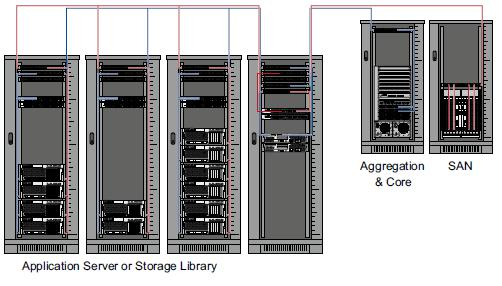
\includegraphics[width=0.5\linewidth]{images/tor_architecture}
\caption{ToR Architektur in der Cisco Variante}
\label{fig:torarchitecture}
\end{figure}


% TODO anz racks
% TODO how many servers per rack
% TODO vorteile nachteile von TOR/EOR. erklären!

\begin{table}[h]
	\centering
	\begin{tabu}{l l l}
		\toprule
		Abteilung & Anzahl Racks & Gesamtzahl Server \\
		\midrule
		HR & 1 & 30 \\
		IT & 1 & 30 \\
		Trading & 1 & 30 \\
		Netzwerk-Switches  & 1 & 5 \\
		\bottomrule
	\end{tabu}
	\caption{Racks und Server je Abteilung}
\end{table}


\subsection{Access Layer}
\paragraph{Physical}
Die Server werden mit je zwei Gigabit Kupfer Kabel beim Access Switch angeschlossen. Die beiden Interfaces bekommen die selbe IP Adresse. Fällt ein Interfaces aus, gibt es ein Failover vom Primary zum Secondary.

\paragraph{Layer 2}
Die Server im Access Layer sind als Looped Triangle organisiert. Dieser Design Ansatz ist weit verbreitet und verfügt über eine schnelle Konvergenz durch RSTP (802.1w) und MSTP (802.1s). Zusätzlich ist es einfach Load Balancer und Firewalls im Aggregation Layer zu deployen. Um Layer 2 Loops zu verhindern wird Rapid PVST+ eingesetzt. Ein Access Switch übernimmt die Funktion des Primary Root und der zweite dient als Backup (Standby). Um die Verfügbarkeit der Standardgateways hoch zu halten, wird das Cisco propertietäre HSRP (Hot Standby Routing Protocol) eingesetzt.  Dabei werden mehrere physische Router zu einer logischen Gruppe zusammengefasst. Fällt ein Switch der logischen Gruppe aus, können die Server stets noch über den Standby Switch auf das Netzwerk zugreifen. 

\paragraph{Layer 3}
Der gesamte Traffic wird bis zum Access Layer mit OSPF geroutet. Dies erlaubt es, die Broadcast Domäne der einzelnen Subnetze so klein wie möglich zu halten.

\subsubsection{3 Tier Organisation im Access Layer}
Alle externen Zugriffe auf die einzelnen Tiers werden mit Firewalls im Aggregation Layer kontrolliert. Der Zugriffsfluss geht grundsätzlich von oben nach unten. Erlaubt sind nur Zugriffe auf den jeweils nächsten Tier. Also WEB $\rightarrow$ Application $\rightarrow$ Database. Die Kommunikation verläuft dann jedoch trotzdem über den Aggregation Layer, der die Zugriffe auf ihre Korrektheit überprüft.
\paragraph{1. WEB Tier} 
Beinhaltet die Webserver

\paragraph{2. Application Tier}
Beinhaltet die bankenspezifischen Services fürs Trading

\paragraph{3. Database Tier}
Beinhaltet alle Datenbanken.

\paragraph{VLAN} \hfill
\begin{table}[h]
	\centering
	\begin{tabu}{l l l}
		\toprule
		VLAN & Subnetz & Beschreibung \\
		\midrule
		21 & 10.200.2.1/26 & Webserver \\
		22 & 10.200.2.65/26 & Application \\
		23 & 10.200.2.129/26 & Database \\
		\bottomrule
	\end{tabu}
	\caption{VLAN's}
\end{table}


\subsection{Aggregation Layer}
Im Aggregation Layer ist die Security Logik (Firewall etc.) implementiert. Die Requests der Server werden über den Access Layer in den Aggregation Layer weitergeleitet und dort auf ihre Gültigkeit überprüft. Unerlaubte Zugriffe auf fremde Netze werden dort von der Firewall blockiert. 


\subsection{Core Layer}
Bei einem Datacenter dieser Grösse ist der Einsatz eines Core Layers von Vorteil. Der Core bündelt die Geräte im Aggregation Layer, was zu einer besseren Skalierbarkeit führt. Ebenfalls kann im Core ein gewisses Load Balancing zwischen dem Campus Core und dem Aggregation Layer implementiert werden. Für das Routing bis zum Access Layer wird OSPF verwendet.  


\subsection{Multitenancy}
Mittels VRF's können die einzelnen Tenands auf Layer 3 voneinander getrennt werden. Somit kann eine strikte Trennung der einzelnen Abteilungen End zu End umgesetzt werden. Auf Layer 2 kann dies zusätzlich mit VLAN's umgesetzt werden. Dies ist jedoch erst ab dem Access Layer nötig.

Eine alternative zu VRF's wäre es, den kompletten Backbone mit MPLS umzusetzen, welches eine saubere Trennung via VPNs erstellt.


\appendix

\section{Konfigurationen}
\label{appendix:configurations}

\subsection{BR1-R1}
\subsubsection{Running Configuration}
\lstinputlisting{appendix/config/br1-r1/br1-r1-config.txt}

\subsubsection{IP Interfaces}
\lstinputlisting{appendix/config/br1-r1/br1-r1-interface.txt}

\subsubsection{Interface Status}
\lstinputlisting{appendix/config/br1-r1/br1-r1-status.txt}

\subsubsection{Neighbors}
\lstinputlisting{appendix/config/br1-r1/br1-r1-neighbors.txt}

\subsection{BR2-R1}
\subsubsection{Running Configuration}
\lstinputlisting{appendix/config/br2-r1/br2-ri-config.txt}

\subsubsection{IP Interfaces}
\lstinputlisting{appendix/config/br2-r1/br2-ri-interface.txt}

\subsubsection{Interface Status}
\lstinputlisting{appendix/config/br2-r1/br2-ri-status.txt}

\subsubsection{Neighbors}
\lstinputlisting{appendix/config/br2-r1/br2-ri-neighbors.txt}

\subsection{BR2-S1}
\subsubsection{Running Configuration}
\lstinputlisting{appendix/config/br2-s1/br2-s1-config.txt}

\subsubsection{IP Interfaces}
\lstinputlisting{appendix/config/br2-s1/br2-s1-interface.txt}

\subsubsection{Interface Status}
\lstinputlisting{appendix/config/br2-s1/br2-s1-status.txt}

\subsubsection{Neighbors}
\lstinputlisting{appendix/config/br2-s1/br2-s1-neighbors.txt}

\subsection{CCNA-CCNP-FRSwitch}
\subsubsection{Running Configuration}
\lstinputlisting{appendix/config/framerelayswitch/framerelayswitch-config.txt}

\subsubsection{IP Interfaces}
\lstinputlisting{appendix/config/framerelayswitch/framerelayswitch-interface.txt}

\subsubsection{Interface Status}
\lstinputlisting{appendix/config/framerelayswitch/framerelayswitch-status.txt}

\subsubsection{Neighbors}
\lstinputlisting{appendix/config/framerelayswitch/framerelayswitch-neighbors.txt}

\subsection{HQ FrameRelay Router (HQ-FRR)}
\subsubsection{Running Configuration}
\lstinputlisting{appendix/config/hq-frr/hq-frr-config.txt}

\subsubsection{IP Interfaces}
\lstinputlisting{appendix/config/hq-frr/hq-frr-interface.txt}

\subsubsection{Interface Status}
\lstinputlisting{appendix/config/hq-frr/hq-frr-status.txt}

\subsubsection{Neighbors}
\lstinputlisting{appendix/config/hq-frr/hq-frr-neighbors.txt}

\subsection{HQ-IER1}
\subsubsection{Running Configuration}
\lstinputlisting{appendix/config/hq-ier1/hq-ier1-config.txt}

\subsubsection{IP Interfaces}
\lstinputlisting{appendix/config/hq-ier1/hq-ier1-interface.txt}

\subsubsection{Interface Status}
\lstinputlisting{appendix/config/hq-ier1/hq-ier1-status.txt}

\subsubsection{Neighbors}
\lstinputlisting{appendix/config/hq-ier1/hq-ier1-neighbors.txt}

\subsection{HQ-WER1}
\subsubsection{Running Configuration}
\lstinputlisting{appendix/config/hq-wer1/hq-wer1-config.txt}

\subsubsection{IP Interfaces}
\lstinputlisting{appendix/config/hq-wer1/hq-wer1-interface.txt}

\subsubsection{Interface Status}
\lstinputlisting{appendix/config/hq-wer1/hq-wer1-status.txt}

\subsubsection{Neighbors}
\lstinputlisting{appendix/config/hq-wer1/hq-wer1-neighbors.txt}

\subsection{HQ CS1}
\subsubsection{Running Configuration}
\lstinputlisting{appendix/config/hq-cs1/hq-cs1-config.txt}

\subsubsection{IP Interfaces}
\lstinputlisting{appendix/config/hq-cs1/hq-cs1-interface.txt}

\subsubsection{Interface Status}
\lstinputlisting{appendix/config/hq-cs1/hq-cs1-status.txt}

\subsubsection{Neighbors}
\lstinputlisting{appendix/config/hq-cs1/hq-cs1-neighbors.txt}

\subsection{HQ CS2}
\subsubsection{Running Configuration}
\lstinputlisting{appendix/config/hq-cs2/hq-cs2-config.txt}

\subsubsection{IP Interfaces}
\lstinputlisting{appendix/config/hq-cs2/hq-cs2-interface.txt}

\subsubsection{Interface Status}
\lstinputlisting{appendix/config/hq-cs2/hq-cs2-status.txt}

\subsubsection{Neighbors}
\lstinputlisting{appendix/config/hq-cs2/hq-cs2-neighbors.txt}

\subsection{HQ CS3}
\subsubsection{Running Configuration}
\lstinputlisting{appendix/config/hq-cs3/hq-cs3-config.txt}

\subsubsection{IP Interfaces}
\lstinputlisting{appendix/config/hq-cs3/hq-cs3-interface.txt}

\subsubsection{Interface Status}
\lstinputlisting{appendix/config/hq-cs3/hq-cs3-status.txt}

\subsubsection{Neighbors}
\lstinputlisting{appendix/config/hq-cs3/hq-cs3-neighbors.txt}

\subsection{HQ CS4}
\subsubsection{Running Configuration}
\lstinputlisting{appendix/config/hq-cs4/hq-cs4-config.txt}

\subsubsection{IP Interfaces}
\lstinputlisting{appendix/config/hq-cs4/hq-cs4-interface.txt}

\subsubsection{Interface Status}
\lstinputlisting{appendix/config/hq-cs4/hq-cs4-status.txt}

\subsubsection{Neighbors}
\lstinputlisting{appendix/config/hq-cs4/hq-cs4-neighbors.txt}

\subsection{HQ DS1}
\subsubsection{Running Configuration}
\lstinputlisting{appendix/config/hq-ds1/hq-ds1-config.txt}

\subsubsection{IP Interfaces}
\lstinputlisting{appendix/config/hq-ds1/hq-ds1-interface.txt}

\subsubsection{Interface Status}
\lstinputlisting{appendix/config/hq-ds1/hq-ds1-status.txt}

\subsubsection{Neighbors}
\lstinputlisting{appendix/config/hq-ds1/hq-ds1-neighbors.txt}

\subsection{HQ DS2}
\subsubsection{Running Configuration}
\lstinputlisting{appendix/config/hq-ds2/hq-ds2-config.txt}

\subsubsection{IP Interfaces}
\lstinputlisting{appendix/config/hq-ds2/hq-ds2-interface.txt}

\subsubsection{Interface Status}
\lstinputlisting{appendix/config/hq-ds2/hq-ds2-status.txt}

\subsubsection{Neighbors}
\lstinputlisting{appendix/config/hq-ds2/hq-ds2-neighbors.txt}

\subsection{HQ DS3}
\subsubsection{Running Configuration}
\lstinputlisting{appendix/config/hq-ds3/hq-ds3-config.txt}

\subsubsection{IP Interfaces}
\lstinputlisting{appendix/config/hq-ds3/hq-ds3-interface.txt}

\subsubsection{Interface Status}
\lstinputlisting{appendix/config/hq-ds3/hq-ds3-status.txt}

\subsubsection{Neighbors}
\lstinputlisting{appendix/config/hq-ds3/hq-ds3-neighbors.txt}


\section{Messungen}
\label{appendix:measures}
\subsection{Von X nach Y}
\lstinputlisting{appendix/config/br2-r1/br2-ri-config.txt}

% Code Listings
% \lstlistoflistings

% List of figures
% \listoffigures

% List of tables
% \listoftables

% Bibliography
% \bibliographystyle{plain} 
% \bibliography{literatur}

\end{document}
